\documentclass[12pt,a4paper,oneside]{book}

\usepackage{styles/rbru_manual}

\begin{document}

% -------------------------------------------------------------
% ส่วนนำ (Front Matter)
% -------------------------------------------------------------
\frontmatter

% 1. หน้าปกคู่มือวิชาการ (Academic Manual Cover)
\begin{titlepage}
    \centering
    \vspace*{0.3cm}
    
    {\fontsize{24}{30}\selectfont\bfseries\color{rbruNavy} มหาวิทยาลัยราชภัฏรำไพพรรณี\par}
    \vspace{0.3cm}
    {\fontsize{17}{22}\selectfont\color{rbruSlate} คณะวิทยาศาสตร์และเทคโนโลยี  สาขาวิชาฟิสิกส์\par}
    {\fontsize{15}{20}\selectfont\color{agriGreen} หน่วยวิจัยเกษตรดิจิทัล JC\_AI\_SciRBRU (Digital Agriphysics \& AI Research Unit)\par}
    
    \vspace{1.0cm}
    {\color{rbruGold}\rule{\textwidth}{2.5pt}\par}
    \vspace{0.5cm}
    
    {\fontsize{22}{28}\selectfont\bfseries\color{rbruNavy} คู่มือการประกอบ ติดตั้ง และใช้งาน\par}
    \vspace{0.4cm}
    {\fontsize{18}{24}\selectfont\bfseries\color{rbruTeal} เครื่องสเปกโทรโฟโตมิเตอร์ตรวจวัดธาตุอาหารหลักในดิน\\และสมบัติเชิงแสงของของเหลว\par}
    \vspace{0.3cm}
    {\fontsize{16}{20}\selectfont\bfseries\color{rbruSlate} NPK Level Meter 1.02 \& Liquid Optics Analyzer\par}
    
    \vspace{0.5cm}
    {\color{rbruGold}\rule{\textwidth}{2.5pt}\par}
    
    \vspace{0.8cm}
    \begin{figure}[H]
        \centering
        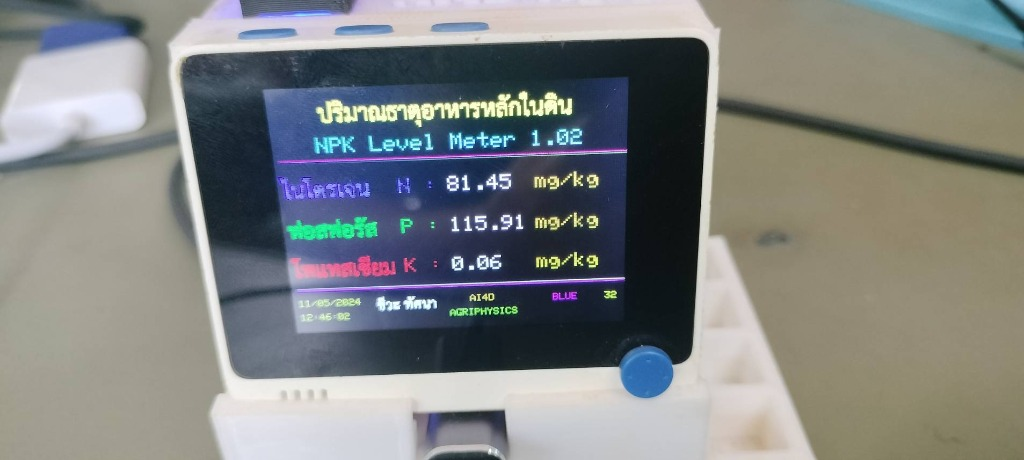
\includegraphics[width=0.62\textwidth]{images/device_overview.jpg}
    \end{figure}
    
    \vfill
    
    {\fontsize{16}{20}\selectfont\bfseries\color{rbruNavy} ผู้ช่วยศาสตราจารย์ ดร.ชีวะ ทัศนา และคณะ\par}
    \vspace{0.2cm}
    {\fontsize{14}{18}\selectfont\color{rbruSlate} เอกสารทางวิชาการและคู่มือการวิจัยและพัฒนาสิ่งประดิษฐ์\par}
    {\fontsize{14}{18}\selectfont\color{rbruSlate} กันยายน 2569\par}
    \vspace*{0.3cm}
\end{titlepage}

% 2. คำนำ (Preface)
\chapter*{คำนำ}
\addcontentsline{toc}{chapter}{คำนำ}

เอกสารคู่มือการประกอบ ติดตั้ง และใช้งานเครื่องสเปกโทรโฟโตมิเตอร์ตรวจวัดธาตุอาหารหลักในดินและสมบัติเชิงแสงของของเหลว (NPK Level Meter 1.02 \& Liquid Optics Analyzer) เล่มนี้ จัดทำขึ้นเพื่อเป็นคู่มือวิชาการและแนวทางการปฏิบัติการเชิงลึก สำหรับนักวิจัย คณาจารย์ นักศึกษา และเกษตรกรผู้สนใจนวัตกรรมเกษตรแม่นยำ (Precision Agriculture) โดยเฉพาะการบริหารจัดการธาตุอาหารในสวนทุเรียนแปลงใหญ่ในเขตภาคตะวันออกของประเทศไทย

ระบบตรวจวัดนี้ได้รับการออกแบบและพัฒนาขึ้นภายใต้แนวคิดการประมวลผลบนชิปสมบูรณ์ (Edge-Only Architecture) โดยผสานสถาปัตยกรรมไมโครคอนโทรลเลอร์สมรรถนะสูง Microchip ATSAMD51 ARM Cortex-M4F ร่วมกับเซนเซอร์วัดค่าสีดิจิทัล TCS34725 และแหล่งกำเนิดแสงสเปกตรัมหลายช่วงคลื่น NeoPixel WS2812B ทำให้สามารถวิเคราะห์ธาตุอาหารดิน ไนโตรเจน (N) ฟอสฟอรัส (P) และโพแทสเซียม (K) ได้อย่างรวดเร็ว พร้อมทั้งรองรับการคำนวณ 3 โหมด คือ โครงข่ายประสาทเทียม TinyML Deep Learning, สมการพหุนามสากล, และระบบสร้างเส้นโค้งมาตรฐานสดในตัวเครื่อง (In-Situ Standard Curve Wizard) ที่คำนวณความชัน จุดตัด $R^2$ LOD และ LOQ ตามเกณฑ์สากลของ IUPAC ตลอดจนการขยายขีดความสามารถสู่หน้าจอที่ 5 เพื่อตรวจวัดดัชนีหักเหของแสง ($n$) ความหนาแน่น ($\rho$) ปริมาณของแข็ง ($^\circ\text{Bx}$) และระดับความขุ่นของตัวอย่างของเหลวทางการเกษตร

เนื้อหาภายในคู่มือเล่มนี้แบ่งออกเป็น 5 บทหลัก และ 2 ภาคผนวก ประกอบด้วย
\begin{enumerate}[leftmargin=1.5em, itemsep=3pt]
    \item \textbf{บทที่ 1 บทนำและหลักการฟิสิกส์เชิงแสง} อธิบายทฤษฎีกฎของเบียร์และแลมเบิร์ต สเปกตรัมการดูดกลืนแสง และแบบจำลองมาตรวิทยาของเหลว
    \item \textbf{บทที่ 2 การออกแบบและประกอบชิ้นส่วนฮาร์ดแวร์} แสดงรายการอุปกรณ์ แผนผังการเชื่อมต่อวงจร และขั้นตอนการประกอบเชิงกล
    \item \textbf{บทที่ 3 การติดตั้งเฟิร์มแวร์และการตั้งค่าซอฟต์แวร์} แนะนำไลบรารีที่จำเป็น การตั้งค่าฟอนต์ภาษาไทย และการคอมไพล์ผ่าน Arduino CLI
    \item \textbf{บทที่ 4 คู่มือการปฏิบัติการและแบบจำลองการเทียบมาตรฐาน} นำเสนอการทำงานของระบบ 5 หน้าจอ ขั้นตอนการวัดดินและของเหลว และสถิติการสร้างกราฟมาตรฐาน
    \item \textbf{บทที่ 5 การบำรุงรักษาและการแก้ไขปัญหา} รวบรวมแนวทางการดูแลรักษาอุปกรณ์และการแก้ไขข้อขัดข้องที่อาจเกิดขึ้นในภาคสนาม
    \item \textbf{ภาคผนวก} รวบรวมตารางค่าดัชนีหักเหและความหนาแน่นมาตรฐาน ICUMSA และข้อมูลจำเพาะเชิงสถาปัตยกรรมของ Wio Terminal
\end{enumerate}

คณะผู้จัดทำหวังเป็นอย่างยิ่งว่า คู่มือวิชาการเล่มนี้จะเป็นประโยชน์ต่อการนำไปประยุกต์ใช้งานจริงในภาคสนาม การจัดการเรียนการสอนในห้องปฏิบัติการฟิสิกส์และเครื่องมือวัด และเป็นรากฐานในการพัฒนาเทคโนโลยีเกษตรอัจฉริยะของประเทศไทยสืบไป

\vspace{1.0cm}
\begin{flushright}
    \begin{minipage}{0.55\textwidth}
        \centering
        \textbf{ผู้ช่วยศาสตราจารย์ ดร.ชีวะ ทัศนา และคณะ}\\
        หน่วยวิจัยฟิสิกส์เพื่อการเกษตรดิจิทัลและปัญญาประดิษฐ์ (AI4D AgriPhysics)\\
        สาขาวิชาฟิสิกส์ คณะวิทยาศาสตร์และเทคโนโลยี\\
        มหาวิทยาลัยราชภัฏรำไพพรรณี\\
        กันยายน 2569
    \end{minipage}
\end{flushright}

\clearpage

% 3. สารบัญหลัก สารบัญภาพ สารบัญตาราง
\phantomsection
\addcontentsline{toc}{chapter}{\contentsname}
\tableofcontents
\clearpage

\phantomsection
\addcontentsline{toc}{chapter}{\listfigurename}
\listoffigures
\clearpage

\phantomsection
\addcontentsline{toc}{chapter}{\listtablename}
\listoftables
\clearpage

% -------------------------------------------------------------
% ส่วนเนื้อหาหลัก (Main Matter - Chapters 1 to 5)
% -------------------------------------------------------------
\mainmatter

\chapter{บทนำและหลักการฟิสิกส์เชิงแสง}
\label{chap:ch01}

\section*{แผนบริหารการสอนประจำบทที่ 1}
\addcontentsline{toc}{section}{แผนบริหารการสอนประจำบทที่ 1}

\begin{planbox}{หัวข้อเนื้อหาประจำบท}
\begin{enumerate}[leftmargin=1.5em, itemsep=1pt]
    \item ความสำคัญของการตรวจวัดธาตุอาหารดินในการเกษตรแม่นยำ
    \item หลักการทางทัศนศาสตร์ฟิสิกส์และกฎของเบียร์และแลมเบิร์ต
    \item การจำแนกแถบสเปกตรัมแสงสำหรับการตรวจวัดธาตุไนโตรเจน ฟอสฟอรัส และโพแทสเซียม
    \item ทฤษฎีการลดทอนแสงและความสัมพันธ์กับดัชนีหักเหและความหนาแน่นของของเหลว
\end{enumerate}
\end{planbox}

\begin{planbox}{วัตถุประสงค์เชิงพฤติกรรม}
\begin{enumerate}[leftmargin=1.5em, itemsep=1pt]
    \item อธิบายหลักการทางฟิสิกส์ของการดูดกลืนแสงตามกฎของเบียร์และแลมเบิร์ตได้อย่างถูกต้อง
    \item จำแนกความยาวคลื่นที่เหมาะสมในการทำปฏิกิริยากับสารละลายธาตุอาหารดินได้อย่างสมบูรณ์
    \item อธิบายความสัมพันธ์ระหว่างการลดทอนแสงกับดัชนีหักเหและความหนาแน่นของของเหลวได้อย่างถูกต้อง
\end{enumerate}
\end{planbox}

\begin{planbox}{กิจกรรมการเรียนการสอน}
\begin{enumerate}[leftmargin=1.5em, itemsep=1pt]
    \item การบรรยายเชิงทฤษฎีประกอบการฉายสื่อแอนิเมชันการแผ่และดูดกลืนคลื่นแม่เหล็กไฟฟ้า
    \item การสาธิตการทำงานของเครื่องสเปกโทรโฟโตมิเตอร์ตรวจวัดสารละลายตัวอย่างจริง
    \item การอภิปรายกลุ่มย่อยเกี่ยวกับการประยุกต์ทัศนศาสตร์ฟิสิกส์ในงานเกษตรดิจิทัล
\end{enumerate}
\end{planbox}

\begin{planbox}{สื่อการเรียนการสอน}
\begin{enumerate}[leftmargin=1.5em, itemsep=1pt]
    \item เอกสารคำสอนและสไลด์บรรยายบทที่ 1
    \item เครื่องสเปกโทรโฟโตมิเตอร์ NPK Level Meter 1.02 และหลอดคิวเวตต์มาตรฐาน
    \item ชุดสารละลายมาตรฐานสีสำหรับการทดสอบการดูดกลืนแสง
\end{enumerate}
\end{planbox}

\begin{planbox}{การวัดและประเมินผล}
\begin{enumerate}[leftmargin=1.5em, itemsep=1pt]
    \item การประเมินความสนใจและการมีส่วนร่วมในการอภิปรายในชั้นเรียน
    \item การทดสอบย่อยวัดความรู้ความเข้าใจเรื่องกฎของเบียร์และแลมเบิร์ต
    \item การตรวจความถูกต้องของการตอบคำถามทบทวนท้ายบทที่ 1
\end{enumerate}
\end{planbox}

\clearpage

\section{ความสำคัญของการตรวจวัดธาตุอาหารดินในการเกษตรแม่นยำ}
การตรวจวัดปริมาณธาตุอาหารหลักในดินอันประกอบด้วยไนโตรเจน ฟอสฟอรัส และโพแทสเซียม หรือ NPK มีความสำคัญอย่างยิ่งต่อการบริหารจัดการธาตุอาหารพืชในการเกษตรแม่นยำ (Precision Agriculture) โดยเฉพาะในพื้นที่ปลูกไม้ผลเศรษฐกิจ เช่น ทุเรียนแปลงใหญ่ การตรวจวัดในภาคสนามที่ต้องการความรวดเร็วและแม่นยำสูงสามารถดำเนินการได้ด้วยเทคนิคการดูดกลืนแสงเชิงสเปกตรัม (Optical Absorption Spectroscopy)

\begin{figure}[H]
    \centering
    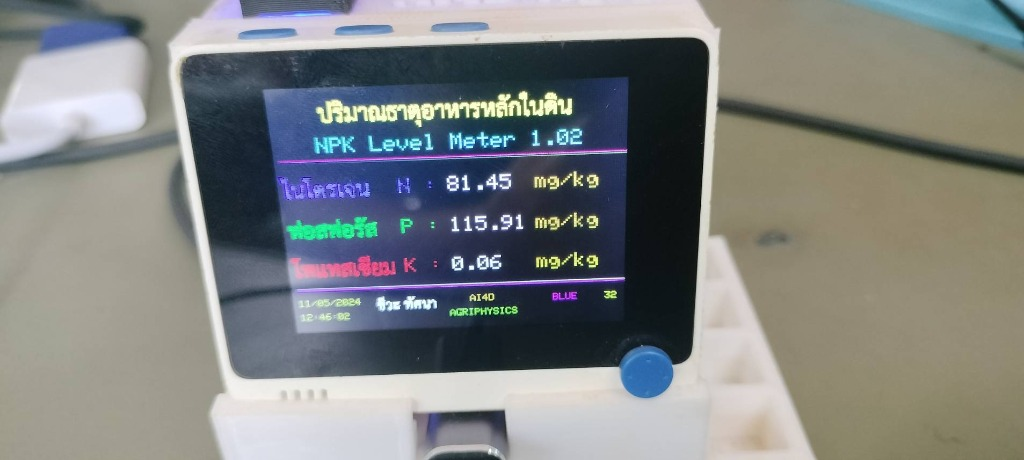
\includegraphics[width=0.70\textwidth]{images/device_overview.jpg}
    \caption{เครื่องสเปกโทรโฟโตมิเตอร์ตรวจวัดธาตุอาหารหลักในดิน NPK Level Meter 1.02}
    \label{fig:device_overview}
\end{figure}

\section{กฎของเบียร์และแลมเบิร์ต}
เมื่อลำแสงเอกรงค์ (Monochromatic Light) หรือแสงที่มีความยาวคลื่นจำเพาะส่องผ่านสารละลายตัวอย่างดินที่ผ่านกระบวนการทำปฏิกิริยาเกิดสี ความเข้มของแสงที่ทะลุผ่านจะลดลงตามความเข้มข้นของสารละลายและความหนาของชั้นสารละลายตามความสัมพันธ์

\begin{equation}
    A(\lambda) = -\log_{10}\left(\frac{I(\lambda) - I_{\text{dark}}}{I_0(\lambda) - I_{\text{dark}}}\right) = \varepsilon(\lambda) \cdot b \cdot C
\end{equation}

กำหนดให้
\begin{itemize}[leftmargin=2.0em, itemsep=2pt]
    \item $A(\lambda)$ แทนค่าการดูดกลืนแสง (Absorbance) ณ ความยาวคลื่น $\lambda$
    \item $I_0(\lambda)$ แทนความเข้มแสงเริ่มต้นที่ส่องผ่านสารละลายแบลงก์ (Blank Reference)
    \item $I(\lambda)$ แทนความเข้มแสงที่ทะลุผ่านสารละลายตัวอย่าง (Sample Transmitted Intensity)
    \item $I_{\text{dark}}$ แทนสัญญาณกระแสมืดของเซนเซอร์ขณะดับไฟ (Dark Current)
    \item $\varepsilon(\lambda)$ แทนสัมประสิทธิ์การดูดกลืนแสงโมลาร์ (Molar Absorptivity)
    \item $b$ แทนความยาวของทางเดินแสงในคิวเวตต์ มีค่าเท่ากับ 1.0 เซนติเมตร
    \item $C$ แทนความเข้มข้นของธาตุอาหารในสารละลาย มีหน่วยเป็นมิลลิกรัมต่อกิโลกรัม ($\text{mg/kg}$)
\end{itemize}

\section{การจำแนกความยาวคลื่นสำหรับการวัด NPK}
ระบบสเปกโทรโฟโตมิเตอร์เครื่องนี้ใช้แหล่งกำเนิดแสงแบบหลายความยาวคลื่นผ่านโมดูลไดโอดเปล่งแสงหลายสีดิจิทัล WS2812B ร่วมกับเซนเซอร์วัดค่าสีแบบดิจิทัล TCS34725 ซึ่งสามารถแยกแยะช่องสัญญาณแสงตามความยาวคลื่นหลักได้ดังนี้

\begin{enumerate}[leftmargin=1.5em, itemsep=3pt]
    \item \textbf{แสงสีน้ำเงิน (Blue Spectrum ความยาวคลื่น 465 นาโนเมตร)} ใช้สำหรับการตรวจวัดความเข้มข้นของธาตุไนโตรเจน (Nitrogen หรือ N) ซึ่งทำปฏิกิริยากับน้ำยาทดสอบเกิดสารประกอบสีส้มอมน้ำตาล
    \item \textbf{แสงสีฟ้าอมเขียว (Cyan Spectrum ความยาวคลื่น 500 นาโนเมตร)} ใช้สำหรับการวิเคราะห์สารประกอบอินทรีย์และการดูดกลืนแสงช่วงกลาง
    \item \textbf{แสงสีเขียว (Green Spectrum ความยาวคลื่น 525 นาโนเมตร)} ใช้สำหรับการตรวจวัดความเข้มข้นของธาตุฟอสฟอรัส (Phosphorus หรือ P) ซึ่งทำปฏิกิริยากับน้ำยาทดสอบเกิดสารประกอบเชิงซ้อนสีน้ำเงินโมลิบดีนัม
    \item \textbf{แสงสีเหลือง (Yellow Spectrum ความยาวคลื่น 590 นาโนเมตร)} ใช้สำหรับการตรวจวัดค่าความขุ่นและอนุภาคแขวนลอยในสารละลาย
    \item \textbf{แสงสีแดง (Red Spectrum ความยาวคลื่น 625 นาโนเมตร)} ใช้สำหรับการตรวจวัดความเข้มข้นของธาตุโพแทสเซียม (Potassium หรือ K) ซึ่งทำให้เกิดความขุ่นและการสะท้อนแสงของตะกอนเตตระฟีนิลบอเรต
    \item \textbf{แสงสีขาว (White Spectrum ความยาวคลื่นครอบคลุม 400 ถึง 700 นาโนเมตร)} ใช้สำหรับการเทียบมาตรฐานศูนย์ (Blank Calibration) และการตรวจวัดค่าความขุ่นรวมของสารละลายดิน
\end{enumerate}

\section{การวิเคราะห์สมบัติเชิงทัศนศาสตร์และมาตรวิทยาของเหลว}
นอกเหนือจากการตรวจวัดธาตุอาหารในดินแล้ว ระบบยังได้รับการพัฒนาขยายขีดความสามารถสู่การเป็นเครื่องตรวจวิเคราะห์สมบัติเชิงแสงและกายภาพของตัวอย่างของเหลวทางการเกษตร (Liquid Optics \& Metrology) เช่น น้ำชลประทาน น้ำหมักชีวภาพ และสารละลายธาตุอาหารพืช โดยอาศัยหลักการความสัมพันธ์ระหว่างการลดทอนแสง (Optical Attenuation) กับดัชนีหักเหของแสง (Refractive Index, $n$) และความหนาแน่นของของเหลว ($\rho$) ตามมาตรฐานสากล ICUMSA และทฤษฎี Lorentz-Lorenz \& Gladstone-Dale

\begin{equation}
    n = 1.3330 + 0.00143 \cdot (\text{Brix}) + 0.0000045 \cdot (\text{Brix})^2
\end{equation}

\begin{equation}
    \rho = 0.9982 + 0.00385 \cdot (\text{Brix}) + 0.000012 \cdot (\text{Brix})^2 \quad (\text{g/cm}^3)
\end{equation}

โดยที่น้ำกลั่นบริสุทธิ์มีค่าดัชนีหักเห $n = 1.3330$ และความหนาแน่น $\rho = 0.9982\text{ g/cm}^3$ ที่อุณหภูมิห้อง 20 องศาเซลเซียส

\section*{บทสรุปประจำบทที่ 1}
\addcontentsline{toc}{section}{บทสรุปประจำบทที่ 1}
การตรวจวัดธาตุอาหารหลักในดิน NPK และสมบัติของเหลวด้วยเทคนิคสเปกโทรโฟโตเมตรี อาศัยหลักการการลดทอนของความเข้มแสงเมื่อส่องผ่านตัวกลางตามกฎของเบียร์และแลมเบิร์ต แหล่งกำเนิดแสงดิจิทัล WS2812B ร่วมกับเซนเซอร์ TCS34725 ช่วยให้สามารถเลือกปล่อยแสงความยาวคลื่นจำเพาะ 465, 500, 525, 590 และ 625 นาโนเมตรได้อย่างแม่นยำ พร้อมทั้งสามารถประเมินสมบัติเชิงกายภาพของของเหลว ทั้งดัชนีหักเห ความหนาแน่น และระดับความเข้มข้นสารละลาย ได้อย่างมีประสิทธิภาพบนอุปกรณ์พกพาขนาดกะทัดรัด

\section*{คำถามทบทวนท้ายบทที่ 1}
\addcontentsline{toc}{section}{คำถามทบทวนท้ายบทที่ 1}
\begin{enumerate}[leftmargin=1.5em, itemsep=3pt]
    \item จงอธิบายหลักการทางฟิสิกส์ของกฎของเบียร์และแลมเบิร์ต และระบุข้อจำกัดในการนำกฎนี้ไปประยุกต์ใช้กับสารละลายตัวอย่างดินที่มีความขุ่นสูง
    \item เหตุใดการตรวจวัดธาตุไนโตรเจน (N) และฟอสฟอรัส (P) จึงต้องใช้ความยาวคลื่นแสงที่แตกต่างกัน จงอธิบายความสัมพันธ์กับสารประกอบเชิงซ้อนที่เกิดขึ้น
    \item สัญญาณกระแสมืด (Dark Current) คืออะไร และเหตุใดระบบเฟิร์มแวร์จึงต้องทำการดับไฟเพื่อวัดกระแสมืดก่อนทำการกวาดสเปกตรัมแสงทุกครั้ง
    \item จงอธิบายความสัมพันธ์ระหว่างค่าการดูดกลืนแสงเฉลี่ย ($A_{\text{mean}}$) ดัชนีหักเห ($n$) และความหนาแน่น ($\rho$) ของของเหลวตามมาตรฐาน ICUMSA
\end{enumerate}

\chapter{การออกแบบและประกอบชิ้นส่วนฮาร์ดแวร์}
\label{chap:ch02}

\section*{แผนบริหารการสอนประจำบทที่ 2}
\addcontentsline{toc}{section}{แผนบริหารการสอนประจำบทที่ 2}

\begin{planbox}{หัวข้อเนื้อหาประจำบท}
\begin{enumerate}[leftmargin=1.5em, itemsep=1pt]
    \item สถาปัตยกรรมฮาร์ดแวร์และคุณสมบัติของไมโครคอนโทรลเลอร์ ATSAMD51
    \item รายการอุปกรณ์และโมดูลตรวจวัดแสง TCS34725 ร่วมกับหลอดไฟ WS2812B
    \item การออกแบบทางเดินแสงของช่องใส่คิวเวตต์เพื่อลดการสะท้อนและการกระเจิง
    \item ขั้นตอนการประกอบกลไกและการต่อขาสัญญาณดิจิทัล
\end{enumerate}
\end{planbox}

\begin{planbox}{วัตถุประสงค์เชิงพฤติกรรม}
\begin{enumerate}[leftmargin=1.5em, itemsep=1pt]
    \item ระบุหน้าที่และตำแหน่งของขาสัญญาณควบคุมในระบบสเปกโทรโฟโตมิเตอร์ได้อย่างถูกต้อง
    \item อธิบายหลักการจัดวางแนวแกนแสงระหว่างแหล่งกำเนิด หลอดคิวเวตต์ และเซนเซอร์ได้อย่างสมบูรณ์
    \item ปฏิบัติการประกอบและทดสอบการเชื่อมต่อวงจรฮาร์ดแวร์ได้อย่างถูกต้องปลอดภัย
\end{enumerate}
\end{planbox}

\begin{planbox}{กิจกรรมการเรียนการสอน}
\begin{enumerate}[leftmargin=1.5em, itemsep=1pt]
    \item การบรรยายและสาธิตการเชื่อมต่อสายสัญญาณผ่านพอร์ต Grove
    \item ปฏิบัติการประกอบชิ้นส่วนฮาร์ดแวร์ลงในกล่องบรรจุ 3D Printed Enclosure
    \item การตรวจสอบความถูกต้องของระบบไฟฟ้าและสัญญาณ I2C ก่อนการจ่ายไฟ
\end{enumerate}
\end{planbox}

\begin{planbox}{สื่อการเรียนการสอน}
\begin{enumerate}[leftmargin=1.5em, itemsep=1pt]
    \item บอร์ด Seeed Studio Wio Terminal พร้อมสายเชื่อมต่อ Grove
    \item โมดูลเซนเซอร์ Adafruit TCS34725 และโมดูลไฟ Grove NeoPixel WS2812B
    \item ชุดโครงสร้างกล่องบรรจุ 3 มิติและแท่นยึดคิวเวตต์ขนาด 10 มิลลิเมตร
\end{enumerate}
\end{planbox}

\begin{planbox}{การวัดและประเมินผล}
\begin{enumerate}[leftmargin=1.5em, itemsep=1pt]
    \item การประเมินทักษะการประกอบวงจรและการจัดสายสัญญาณอย่างเป็นระเบียบ
    \item การทดสอบการตรวจพบอุปกรณ์ I2C ผ่านโปรแกรมตรวจสอบที่อยู่บัส
    \item การตรวจความถูกต้องของการตอบคำถามทบทวนท้ายบทที่ 2
\end{enumerate}
\end{planbox}

\clearpage

\section{รายการอุปกรณ์และโมดูลฮาร์ดแวร์}
อุปกรณ์ที่ใช้ในการประกอบและสร้างเครื่องสเปกโทรโฟโตมิเตอร์ประกอบด้วยรายการดังแสดงในตารางที่ \ref{tab:components}

\begin{table}[H]
    \caption{รายการอุปกรณ์และโมดูลฮาร์ดแวร์}
    \label{tab:components}
    \begin{tabularx}{\textwidth}{p{3.2cm}p{4.2cm}X}
        \toprule
        \textbf{อุปกรณ์} & \textbf{รุ่นหรือรหัสสินค้า} & \textbf{บทบาทหน้าที่ในระบบ} \\
        \midrule
        บอร์ดประมวลผล & Seeed Studio Wio Terminal & ไมโครคอนโทรลเลอร์ ATSAMD51 พร้อมจอ LCD 2.4 นิ้ว \\
        เซนเซอร์ตรวจวัดแสง & Adafruit TCS34725 & เซนเซอร์ตรวจวัดแสงสีและค่าความสว่างแบบ I2C \\
        แหล่งกำเนิดแสงสี & Grove RGB LED (WS2812B) & ไดโอดเปล่งแสงควบคุมสีแบบดิจิทัลความยาวคลื่นแม่นยำ \\
        ช่องใส่หลอดทดลอง & Cuvette Holder 10 mm & แท่นยึดหลอดคิวเวตต์มาตรฐานทางเดินแสง 10 มิลลิเมตร \\
        สายเชื่อมต่อข้อมูล & Grove 4-Pin Cable & สายส่งสัญญาณดิจิทัลและสายจ่ายพลังงานไฟฟ้า \\
        การ์ดหน่วยความจำ & microSD Card Class 10 & อุปกรณ์บันทึกผลการวัดลงไฟล์ข้อมูล 4 รูปแบบ (NPK.csv, SPECTRUM.csv, CALIB\_LOG.csv, LIQUID\_LOG.csv) \\
        โครงสร้างตัวเครื่อง & 3D Printed Enclosure & กล่องบรรจุอุปกรณ์ภายนอกออกแบบด้วยเส้นใย PLA+ \\
        \bottomrule
    \end{tabularx}
\end{table}

\section{แผนภาพการต่อวงจรและขาสัญญาณ}
การเชื่อมต่อสัญญาณระหว่างบอร์ด Wio Terminal กับโมดูลเซนเซอร์และแหล่งกำเนิดแสง แสดงรายละเอียดตามตารางที่ \ref{tab:pinout}

\begin{table}[H]
    \caption{การกำหนดขาสัญญาณและการเชื่อมต่ออุปกรณ์}
    \label{tab:pinout}
    \begin{tabularx}{\textwidth}{p{3.0cm}p{3.0cm}p{3.0cm}X}
        \toprule
        \textbf{อุปกรณ์ภายนอก} & \textbf{พอร์ต Wio Terminal} & \textbf{ขาสัญญาณไมโคร} & \textbf{คำอธิบายการเชื่อมต่อ} \\
        \midrule
        TCS34725 (SDA) & Grove พอร์ตขวา & ขา SDA (PA17) & ส่งสัญญาณข้อมูล I2C บัสความเร็ว 100 kHz \\
        TCS34725 (SCL) & Grove พอร์ตขวา & ขา SCL (PA16) & ส่งสัญญาณนาฬิกา I2C บัสความเร็ว 100 kHz \\
        TCS34725 (VCC) & Grove พอร์ตขวา & ขา 3V3 หรือ 5V & แหล่งจ่ายพลังงานไฟฟ้ากระแสตรง 3.3 โวลต์ \\
        TCS34725 (GND) & Grove พอร์ตขวา & ขา GND & กราวด์ร่วมของระบบ \\
        \midrule
        RGB LED (DIN)  & Grove พอร์ตซ้าย & ขา D0 (PB08) & ขาสัญญาณข้อมูลควบคุมหลอด NeoPixel WS2812B \\
        RGB LED (VCC)  & Grove พอร์ตซ้าย & ขา 5V        & จ่ายแรงดันไฟฟ้าเลี้ยงหลอดไฟ 5 โวลต์ \\
        RGB LED (GND)  & Grove พอร์ตซ้าย & ขา GND       & กราวด์ร่วมของหลอดไฟ \\
        \midrule
        ปุ่มกด A       & ด้านบนตัวเครื่อง & WIO\_KEY\_A (28) & ปุ่มด้านขวาสุด ควบคุมการเปิดปิดแสงสีแดง \\
        ปุ่มกด B       & ด้านบนตัวเครื่อง & WIO\_KEY\_B (29) & ปุ่มตรงกลาง ควบคุมการเปิดปิดแสงสีเขียว \\
        ปุ่มกด C       & ด้านบนตัวเครื่อง & WIO\_KEY\_C (30) & ปุ่มด้านซ้ายสุด ควบคุมการเปิดปิดแสงสีน้ำเงิน \\
        จอยสติ๊กกลาง   & ด้านหน้าตัวเครื่อง & WIO\_5S\_PRESS (35) & กดลงตรงกลาง ควบคุมการเปิดปิดแสงสีขาว \\
        \bottomrule
    \end{tabularx}
\end{table}

\section{การออกแบบทางเดินแสงและกล่องบรรจุ 3 มิติ}
กล่องบรรจุอุปกรณ์ภายนอก (Enclosure) และแท่นยึดคิวเวตต์ได้รับการขึ้นรูปด้วยเครื่องพิมพ์สามมิติ (3D Printing) โดยใช้วัสดุเส้นใย PLA+ สีดำด้าน (Matte Black) เพื่อลดการสะท้อนแสงภายในห้องวัด (Internal Reflection Reduction) โดยมีคุณลักษณะทางทัศนศาสตร์ที่สำคัญ
\begin{itemize}[leftmargin=1.5em, itemsep=2pt]
    \item \textbf{แนวแกนแสงตรง (Coaxial Optical Path):} กึ่งกลางหลอดไฟ WS2812B ช่องคิวเวตต์ และเซนเซอร์ TCS34725 อยู่ในระดับความสูงเดียวกันที่ 15.0 มิลลิเมตรจากฐาน
    \item \textbf{ช่องจำกัดลำแสง (Collimating Aperture):} ขนาดเส้นผ่านศูนย์กลาง 3.0 มิลลิเมตร ติดตั้งระหว่างหลอด LED กับผิวคิวเวตต์ เพื่อให้ได้ลำแสงขนานที่ตั้งฉากกับผนังคิวเวตต์
    \item \textbf{ฝาครอบกันแสงภายนอก (Light-Tight Lid):} มีขอบประกบแบบเขี้ยวซ้อน (Baffle Joint) ป้องกันแสงรอบข้าง (Ambient Light Stray) เล็ดลอดเข้าสู่เซนเซอร์ได้อย่างสมบูรณ์
\end{itemize}

\section{ขั้นตอนการประกอบชิ้นส่วนกลไก}
การประกอบอุปกรณ์ลงในกล่องบรรจุ 3D Printed Enclosure มีขั้นตอนดังต่อไปนี้

\begin{enumerate}[leftmargin=1.5em, itemsep=3pt]
    \item นำแท่นยึดหลอดคิวเวตต์ (Cuvette Holder) ติดตั้งเข้ากับฐานล่างของกล่อง โดยหันด้านช่องส่องแสงให้ตรงกับตำแหน่งติดตั้งโมดูลหลอดไฟและเซนเซอร์
    \item ติดตั้งโมดูลหลอดไฟ Grove RGB LED เข้ากับด้านข้างช่องคิวเวตต์ โดยให้ผิวหน้าของหลอด LED ขนานกับผนังคิวเวตต์และกั้นแสงรบกวนจากภายนอก
    \item ติดตั้งโมดูลเซนเซอร์ TCS34725 ในตำแหน่งตรงข้ามกับหลอด LED ในแนวแกนแสงเดียวกัน เพื่อให้รับลำแสงที่ทะลุผ่านหลอดคิวเวตต์ได้อย่างสมบูรณ์
    \item เสียบสาย Grove 4-Pin จากหลอด LED เข้าสู่พอร์ต Grove ด้านซ้าย (D0) ของบอร์ด Wio Terminal
    \item เสียบสาย Grove 4-Pin จากเซนเซอร์ TCS34725 เข้าสู่พอร์ต Grove ด้านขวา (I2C) ของบอร์ด Wio Terminal
    \item ประกอบบอร์ด Wio Terminal เข้ากับฝาครอบด้านหน้า ขันสกรูยึดให้แน่นหนา และตรวจเช็คการขยับของปุ่มกด A, B, C และจอยสติ๊กด้านหน้าให้เคลื่อนไหวได้อย่างอิสระ
\end{enumerate}

\section*{บทสรุปประจำบทที่ 2}
\addcontentsline{toc}{section}{บทสรุปประจำบทที่ 2}
การออกแบบโครงสร้างฮาร์ดแวร์ของเครื่องสเปกโทรโฟโตมิเตอร์คำนึงถึงความแม่นยำทางทัศนศาสตร์และความสะดวกในการพกพา การใช้พอร์ต Grove อำนวยความสะดวกในการเชื่อมต่อเซนเซอร์ I2C และหลอดดิจิทัล NeoPixel อย่างแน่นหนา ในขณะที่ห้องวัดแสงที่พิมพ์ด้วยเส้นใยสีดำด้านพร้อมช่องจำกัดลำแสงช่วยลดสัญญาณรบกวนและแสงกระเจิง ส่งผลให้สัญญาณการวัดมีความเสถียรและทำซ้ำได้สูง

\section*{คำถามทบทวนท้ายบทที่ 2}
\addcontentsline{toc}{section}{คำถามทบทวนท้ายบทที่ 2}
\begin{enumerate}[leftmargin=1.5em, itemsep=3pt]
    \item เหตุใดการออกแบบแท่นยึดคิวเวตต์จึงต้องใช้วัสดุสีดำด้าน และหากใช้วัสดุสีขาวสะท้อนแสงจะส่งผลกระทบต่อค่าการดูดกลืนแสงอย่างไร
    \item สัญญาณนาฬิกา I2C ที่ความเร็ว 100 kHz เหมาะสมกับการอ่านค่าจากเซนเซอร์ TCS34725 หรือไม่ เพราะเหตุใด
    \item จงอธิบายบทบาทของช่องจำกัดลำแสง (Collimating Aperture) ที่อยู่ระหว่างหลอดไฟ LED กับคิวเวตต์
    \item หากเซนเซอร์ TCS34725 ไม่อยู่ในแนวแกนเดียวกับหลอด LED จะเกิดความคลาดเคลื่อนเชิงแสงในลักษณะใด
\end{enumerate}

\section{การติดตั้งเฟิร์มแวร์และการตั้งค่าซอฟต์แวร์}
\label{sec:firmware}

เฟิร์มแวร์ของเครื่องสเปกโทรโฟโตมิเตอร์พัฒนาขึ้นบนระบบนิเวศ Arduino โดยปรับแต่งให้ทำงานบนสถาปัตยกรรม ARM Cortex-M4F ของไมโครคอนโทรลเลอร์ ATSAMD51 บนบอร์ด Seeed Studio Wio Terminal พร้อมระบบบริหารจัดการหน่วยความจำและจอแสดงผลที่มีประสิทธิภาพสูง

\subsection{ไลบรารีที่จำเป็นสำหรับระบบ}
การพัฒนาและคอมไพล์โปรแกรมต้องการไลบรารีมาตรฐานดังต่อไปนี้

\begin{enumerate}
    \item \textbf{Seeed\_Arduino\_LCD} ไลบรารีควบคุมจอแสดงผล TFT LCD ความละเอียด 320x240 พิกเซลผ่านบัส SPI3 เฉพาะตัวของ Wio Terminal
    \item \textbf{Adafruit\_TCS34725} ไลบรารีสื่อสารกับเซนเซอร์วัดค่าสีแบบ I2C ควบคุมเวลาการประมวลผล (Integration Time) และเกนขยายสัญญาณ
    \item \textbf{Adafruit\_NeoPixel} ไลบรารีขับสัญญาณดิจิทัลควบคุมโมดูลหลอดไฟ RGB WS2812B
    \item \textbf{Seeed\_Arduino\_FS และ Seeed\_SD} ไลบรารีจัดการระบบไฟล์และบันทึกข้อมูลลงในการ์ดหน่วยความจำ microSD Card
\end{enumerate}

\subsection{ข้อควรระวังสำคัญด้านไลบรารีจอแสดงผล}
\begin{academicbox}{การป้องกันปัญหาจอขาวและการตั้งค่าไลบรารี}
    ในการคอมไพล์โปรแกรมสำหรับบอร์ด Wio Terminal จะต้องใช้ไลบรารี \textbf{Seeed\_Arduino\_LCD} ที่ติดตั้งมาพร้อมกับ Core Seeeduino SAMD เท่านั้น โดยห้ามใช้ไลบรารี TFT\_eSPI ทั่วไปของ Bodmer เนื่องจากมีการกำหนดขาสัญญาณ SPI ผิดพลาดและส่งผลให้จอแสดงผลเป็นสีขาวสว่างค้าง
    
    นอกจากนี้ เพื่อให้ระบบสามารถแสดงผลฟอนต์ภาษาไทย THSarabunPSK ได้อย่างคมชัด จะต้องเปิดการทำงานของคุณสมบัติ Smooth Font ในไฟล์ \texttt{User\_Setup.h} ของ Seeed\_Arduino\_LCD โดยเปิดใช้งานบรรทัด:
    \begin{center}
        \texttt{\#define SMOOTH\_FONT}
    \end{center}
\end{academicbox}

\subsection{คำสั่งคอมไพล์และอัปโหลดโปรแกรม}
ผู้ใช้งานสามารถคอมไพล์และอัปโหลดโปรแกรมผ่านโปรแกรม Arduino CLI บนระบบปฏิบัติการ macOS หรือ Linux โดยใช้ชุดคำสั่งดังต่อไปนี้

\begin{center}
\begin{minipage}{0.92\textwidth}
\begin{verbatim}
# Compile sketch for Wio Terminal
arduino-cli compile --fqbn Seeeduino:samd:seeed_wio_terminal firmware

# Upload sketch via USB port
arduino-cli upload -p /dev/cu.usbmodem2101 \
    --fqbn Seeeduino:samd:seeed_wio_terminal firmware
\end{verbatim}
\end{minipage}
\end{center}

กรณีที่เกิดปัญหาพอร์ต USB หลุดการเชื่อมต่อ สามารถแก้ไขได้โดยการเลื่อนสวิตช์เปิดปิดด้านข้างตัวเครื่องลง 2 ครั้งอย่างรวดเร็ว (Double-click Touch Reset) เพื่อเข้าสู่โหมด Bootloader จากนั้นคัดลอกไฟล์ไบนารี \texttt{spectrometer\_npk2026.uf2} ไปวางในไดรฟ์ USB ที่ปรากฏขึ้นได้อย่างสะดวก

\chapter{คู่มือการปฏิบัติการและแบบจำลองการเทียบมาตรฐาน}
\label{chap:ch04}

\section*{แผนบริหารการสอนประจำบทที่ 4}
\addcontentsline{toc}{section}{แผนบริหารการสอนประจำบทที่ 4}

\begin{planbox}{หัวข้อเนื้อหาประจำบท}
\begin{enumerate}[leftmargin=1.5em, itemsep=1pt]
    \item สถาปัตยกรรมการสลับหน้าจอ 5 หน้าจอ (5-Screen Carousel UI)
    \item ระบบการวิเคราะห์ 3 โหมด: TinyML, แบบจำลองพหุนาม และเส้นโค้งมาตรฐานสด
    \item ทฤษฎีการถดถอยเชิงเส้นตรง OLS การประเมินค่า $R^2$, LOD และ LOQ
    \item การวิเคราะห์สมบัติเชิงแสงและความหนาแน่นของของเหลวตามเกณฑ์ ICUMSA
    \item ขั้นตอนการตรวจวัดตัวอย่างดินและของเหลวในภาคสนาม และการบันทึกข้อมูล 4 ไฟล์
\end{enumerate}
\end{planbox}

\begin{planbox}{วัตถุประสงค์เชิงพฤติกรรม}
\begin{enumerate}[leftmargin=1.5em, itemsep=1pt]
    \item อธิบายขั้นตอนการสลับหน้าจอและการควบคุมคำสั่งผ่านจอยสติ๊กได้อย่างถูกต้อง
    \item คำนวณค่าสถิติการถดถอย $m$, $c$, $R^2$, LOD และ LOQ ได้อย่างถูกต้องตามเกณฑ์ IUPAC
    \item ปฏิบัติการตรวจวัดธาตุอาหารดินและสมบัติของเหลวได้อย่างถูกต้อง แม่นยำ
\end{enumerate}
\end{planbox}

\begin{planbox}{กิจกรรมการเรียนการสอน}
\begin{enumerate}[leftmargin=1.5em, itemsep=1pt]
    \item การสาธิตการใช้งานเครื่องสเปกโทรโฟโตมิเตอร์ครบทั้ง 5 หน้าจอ
    \item ปฏิบัติการสร้างเส้นโค้งมาตรฐาน 5 จุดความเข้มข้นสารละลาย NPK
    \item ปฏิบัติการสแกนสเปกตรัมของเหลวตัวอย่างและวิเคราะห์ดัชนีหักเหและความหนาแน่น
\end{enumerate}
\end{planbox}

\begin{planbox}{สื่อการเรียนการสอน}
\begin{enumerate}[leftmargin=1.5em, itemsep=1pt]
    \item เครื่องสเปกโทรโฟโตมิเตอร์ Wio Terminal และการ์ด microSD
    \item ชุดสารละลายมาตรฐาน N, P, K ความเข้มข้น 0, 20, 40, 80, 160 mg/kg
    \item สารละลายตัวอย่างของเหลวและน้ำกลั่นบริสุทธิ์สำหรับเทียบศูนย์
\end{enumerate}
\end{planbox}

\begin{planbox}{การวัดและประเมินผล}
\begin{enumerate}[leftmargin=1.5em, itemsep=1pt]
    \item การประเมินทักษะการเทียบศูนย์และการปฏิบัติการสแกนสเปกตรัม
    \item การตรวจสอบความถูกต้องของไฟล์ข้อมูล NPK.csv, CALIB\_LOG.csv และ LIQUID\_LOG.csv
    \item การตรวจความถูกต้องของการตอบคำถามทบทวนท้ายบทที่ 4
\end{enumerate}
\end{planbox}

\clearpage

\section{ระบบควบคุมหน้าจอและการนำทาง}
การใช้งานเครื่องสเปกโทรโฟโตมิเตอร์ตรวจวัดธาตุอาหารในดิน NPK Level Meter 1.02 ได้รับการออกแบบสถาปัตยกรรมซอฟต์แวร์ให้รองรับระบบเมนู 5 หน้าจอหลัก (5-Screen Carousel UI) ดังแสดงในตารางที่ \ref{tab:controls_mapping}

\begin{table}[H]
\centering
\caption{ฟังก์ชันการควบคุมการนำทางและคำสั่งของตัวเครื่อง}
\label{tab:controls_mapping}
\begin{tabularx}{\textwidth}{p{3.5cm}p{2.2cm}X}
\toprule
\textbf{ปุ่มกด / จอยสติ๊ก} & \textbf{ตำแหน่ง} & \textbf{หน้าที่การทำงาน} \\
\midrule
จอยสติ๊กโยกซ้าย (\texttt{WIO\_5S\_LEFT}) & ด้านหน้า & สลับไปยังหน้าจอก่อนหน้า (Page Loop 1 $\leftrightarrow$ 5) \\
จอยสติ๊กโยกขวา (\texttt{WIO\_5S\_RIGHT}) & ด้านหน้า & สลับไปยังหน้าจอถัดไป \\
จอยสติ๊กโยกลง (\texttt{WIO\_5S\_DOWN}) & ด้านหน้า & หน้าสเปกตรัม: สั่ง \textbf{Auto-Scan} กวาดแสง \\
 & & หน้าคาลิเบรต: สั่ง \textbf{บันทึกจุดสารมาตรฐาน (Step Calib)} \\
 & & หน้าของเหลว: สั่ง \textbf{วิเคราะห์สมบัติของเหลว (Analyze)} \\
จอยสติ๊กโยกขึ้น (\texttt{WIO\_5S\_UP}) & ด้านหน้า & หน้า NPK: สลับโหมดคำนวณ \textbf{[AI] $\to$ [PL] $\to$ [SC]} \\
จอยสติ๊กกดตรงกลาง (\texttt{WIO\_5S\_PRESS}) & ด้านหน้า & หน้าคาลิเบรต / ของเหลว: สั่ง \textbf{Zero Blank ($I_0$)} เทียบน้ำกลั่น \\
 & & หน้าอื่น: เปิดหรือปิดสลับกันของ \textbf{แสงสีขาว (White LED)} \\
ปุ่ม C (ซ้ายสุดด้านบน) & ด้านบน & หน้าคาลิเบรต: เลือกคาลิเบรต \textbf{ไนโตรเจน (N - 465 nm)} \\
 & & หน้า NPK: เปิดหรือปิดสลับกันของ \textbf{แสงสีน้ำเงิน (Blue LED)} \\
ปุ่ม B (กลางด้านบน) & ด้านบน & หน้าคาลิเบรต: เลือกคาลิเบรต \textbf{ฟอสฟอรัส (P - 525 nm)} \\
 & & หน้า NPK: เปิดหรือปิดสลับกันของ \textbf{แสงสีเขียว (Green LED)} \\
ปุ่ม A (ขวาสุดด้านบน) & ด้านบน & หน้าคาลิเบรต: เลือกคาลิเบรต \textbf{โพแทสเซียม (K - 625 nm)} \\
 & & หน้า NPK: เปิดหรือปิดสลับกันของ \textbf{แสงสีแดง (Red LED)} \\
\bottomrule
\end{tabularx}
\end{table}

\section{ระบบประมวลผลการคำนวณ 3 รูปแบบ}
ในหน้าจอตรวจวัด NPK Level Meter ผู้ใช้งานสามารถกดโยกจอยสติ๊กขึ้นเพื่อสลับโหมดการคำนวณได้ 3 รูปแบบอย่างอิสระ
\begin{enumerate}[leftmargin=1.5em, itemsep=3pt]
    \item \textbf{โหมดปัญญาประดิษฐ์ [AI] (TinyML Deep Neural Network)} ใช้โครงข่ายประสาทเทียม Multi-Layer Perceptron ($6 \to 12 \to 8 \to 3$) ประมวลผลบนฮาร์ดแวร์ FPU พร้อมระบบชดเชยความขุ่นของสารละลายดิน (Turbidity Matrix Compensation)
    \item \textbf{โหมดพหุนามสากล [PL] (Classical Literature Polynomial)} คำนวณความเข้มข้นจากสัดส่วนแสงสัมพัทธ์ $r_p, g_p, b_p$ ตามแบบจำลองพหุนามดั้งเดิม
    \item \textbf{โหมดเส้นโค้งมาตรฐานสด [SC] (In-Situ Calibrated Standard Curve)} คำนวณความเข้มข้นจากสมการเส้นตรงที่ผู้ใช้วัดเทียบสดในแปลงเกษตรด้วยสารละลายมาตรฐาน
    \begin{equation}
        C_{\text{sample}} = \max\left(0.0, \, \frac{A_{\text{sample}} - c}{m}\right)
    \end{equation}
\end{enumerate}

\section{ทฤษฎีการถดถอยเชิงเส้นและมาตรวิทยาเคมีวิเคราะห์}
ระบบเฟิร์มแวร์ของ Wio Terminal ได้รับการพัฒนาให้มีระบบวิเคราะห์การถดถอยกำลังสองน้อยที่สุด (Ordinary Least Squares หรือ OLS) บนชิป SAMD51 โดยตรง จากคู่ลำดับความเข้มข้นและค่าการดูดกลืนแสงของสารมาตรฐาน 5 จุด ($C_i, A_i$) สำหรับ $C \in \{0, 20, 40, 80, 160\}\text{ mg/kg}$

\subsection{ความชัน จุดตัดแกน และสัมประสิทธิ์การตัดสินใจ}
\begin{align}
    m &= \frac{\sum_{i=1}^N (C_i - \bar{C})(A_i - \bar{A})}{\sum_{i=1}^N (C_i - \bar{C})^2} \\
    c &= \bar{A} - m \bar{C} \\
    R^2 &= \frac{\left[\sum_{i=1}^N (C_i - \bar{C})(A_i - \bar{A})\right]^2}{\sum_{i=1}^N (C_i - \bar{C})^2 \sum_{i=1}^N (A_i - \bar{A})^2}
\end{align}

\subsection{ขีดจำกัดการตรวจวัดและขีดจำกัดการหาปริมาณ}
ความคลาดเคลื่อนมาตรฐานของส่วนตกค้าง ($s_{y/x}$) คำนวณจาก
\begin{equation}
    s_{y/x} = \sqrt{\frac{\sum_{i=1}^N \left(A_i - (m C_i + c)\right)^2}{N - 2}}
\end{equation}

จากนั้นประเมินขีดจำกัดการตรวจวัด (Limit of Detection หรือ LOD) และขีดจำกัดการหาปริมาณ (Limit of Quantification หรือ LOQ) ตามเกณฑ์สากลของ IUPAC
\begin{align}
    \text{LOD} &= \frac{3.3 \cdot s_{y/x}}{m} \\
    \text{LOQ} &= \frac{10.0 \cdot s_{y/x}}{m}
\end{align}

\section{การตรวจวัดสเปกตรัมการดูดกลืนแสงหลายช่วงคลื่น}
ในหน้าจอที่ 3 ผู้ใช้งานสามารถกดโยกจอยสติ๊กลง (\texttt{WIO\_5S\_DOWN}) เพื่อสั่ง Auto-Scan ระบบจะทำการดับไฟ 50 ms เพื่ออ่านค่ากระแสมืด ($I_{\text{dark}}$) แล้วกวาดแสง 5 ช่วงความยาวคลื่น (465, 500, 525, 590, 625 nm) พร้อมพล็อตกราฟเส้น $A(\lambda)$ แสดงจุดมาร์กเกอร์และตำแหน่งพีคการดูดกลืนแสง ($\lambda_{\max}, A_{\max}$) หากค่าการดูดกลืนแสงสูงเกิน 1.50 ระบบจะแสดงสัญญาณเตือนความเข้มข้นสูงเกินย่านเชิงเส้นทันที

\section{การวิเคราะห์สมบัติเชิงทัศนศาสตร์และความหนาแน่นของของเหลว}
ในหน้าจอที่ 5 ผู้ใช้งานสามารถตรวจวิเคราะห์สมบัติเชิงแสงและกายภาพของตัวอย่างของเหลว (Liquid Optics \& Metrology) ได้อย่างละเอียด ประกอบด้วย
\begin{enumerate}[leftmargin=1.5em, itemsep=3pt]
    \item \textbf{ดัชนีหักเหของของเหลว (Refractive Index, $n$)} คำนวณจากความสัมพันธ์เชิงทัศนศาสตร์ของสารละลายตามมาตรฐานสากล ICUMSA
    \begin{equation}
        n = 1.3330 + 0.00143 \cdot (\text{Brix}) + 0.0000045 \cdot (\text{Brix})^2
    \end{equation}
    โดยที่ $n_{\text{water}} = 1.3330$ ที่อุณหภูมิห้อง 20 องศาเซลเซียส
    \item \textbf{ความหนาแน่นของของเหลว (Density, $\rho$)} คำนวณตามแบบจำลอง Lorentz-Lorenz และ Gladstone-Dale ในหน่วย $\text{g/cm}^3$
    \begin{equation}
        \rho = 0.9982 + 0.00385 \cdot (\text{Brix}) + 0.000012 \cdot (\text{Brix})^2
    \end{equation}
    \item \textbf{ความเข้มข้นสารละลายและน้ำตาล (Brix Degree, $^\circ\text{Bx}$)} ประเมินจากการลดทอนความเข้มแสงและการดูดกลืนแสงเฉลี่ย ($A_{\text{mean}}$)
    \begin{equation}
        \text{Brix} = A_{\text{mean}} \times 26.5
    \end{equation}
    \item \textbf{ความส่องผ่านแสง (\%T) และการจำแนกความขุ่น (Clarity)}
    ระบบจะจำแนกสถานะความขุ่นออกเป็น 3 ระดับ
    \begin{itemize}[leftmargin=1.5em, itemsep=2pt]
        \item \textbf{CLEAR (ใส)} เมื่อค่าการดูดกลืนแสงเฉลี่ย $A < 0.12$
        \item \textbf{SLIGHT TURBID (ขุ่นเบา)} เมื่อ $0.12 \le A < 0.38$
        \item \textbf{TURBID (ขุ่นแขวนลอย)} เมื่อ $A \ge 0.38$
    \end{itemize}
\end{enumerate}

\section{ขั้นตอนการปฏิบัติการตรวจวัดในภาคสนาม}
\subsection{ขั้นตอนการตรวจวัดธาตุอาหารดิน}
\begin{enumerate}[leftmargin=1.5em, itemsep=2pt]
    \item ชั่งตัวอย่างดินแห้ง 5 กรัม ผสมน้ำยาสกัดธาตุอาหาร เขย่า 5 นาที และตั้งทิ้งไว้ให้ตกตะกอนใส
    \item ดูดสารละลายใส 2 มิลลิลิตร ใส่หลอดทดลองและเติมน้ำยาทดสอบเฉพาะของ N, P หรือ K
    \item เทียบศูนย์แบลงก์ด้วยน้ำกลั่นในหน้า Calibrate โดยกดจอยสติ๊กตรงกลาง (\texttt{WIO\_5S\_PRESS})
    \item ใส่หลอดคิวเวตต์บรรจุสารตัวอย่างลงในช่องวัด ปิดฝากันแสง และอ่านค่า NPK บนหน้าจอ
\end{enumerate}

\subsection{ขั้นตอนการตรวจวัดสมบัติของเหลว}
\begin{enumerate}[leftmargin=1.5em, itemsep=2pt]
    \item เลื่อนไปหน้าจอที่ 5 (\texttt{PAGE\_LIQUID})
    \item บรรจุน้ำกลั่นบริสุทธิ์ลงในคิวเวตต์ ใส่ในช่องวัด และกดจอยสติ๊กตรงกลางเพื่อตั้งค่าอ้างอิงน้ำกลั่น
    \item เปลี่ยนเป็นตัวอย่างของเหลวที่ต้องการตรวจวัด และกดจอยสติ๊กลง (\texttt{WIO\_5S\_DOWN})
    \item อ่านค่าดัชนีหักเห $n$, ความหนาแน่น $\rho$, Brix และระดับความขุ่นบนหน้าจอ
\end{enumerate}

\section{สถาปัตยกรรมการบันทึกข้อมูลบน microSD Card}
ระบบทำการบันทึกข้อมูลลง microSD Card แบบ Quadruple Logging 4 ไฟล์หลัก
\begin{itemize}[leftmargin=1.5em, itemsep=2pt]
    \item \texttt{NPK.csv} บันทึกค่าความเข้มข้น N, P, K ต่อเนื่องทุกวินาที
    \item \texttt{SPECTRUM.csv} บันทึกค่า Absorbance สเปกตรัม 5 ย่านคลื่นเมื่อสั่ง Auto-Scan
    \item \texttt{CALIB\_LOG.csv} บันทึกประวัติสมการเส้นตรงมาตรฐาน $R^2$, ความชัน $m$, จุดตัด $c$, LOD, LOQ
    \item \texttt{LIQUID\_LOG.csv} บันทึกผลการวิเคราะห์สมบัติเชิงแสงและความหนาแน่นของเหลว
\end{itemize}

\section*{บทสรุปประจำบทที่ 4}
\addcontentsline{toc}{section}{บทสรุปประจำบทที่ 4}
ระบบซอฟต์แวร์ 5 หน้าจอของ Wio Terminal ผสานการทำงานระหว่างการตรวจวัดธาตุอาหารดินแบบเรียลไทม์ การสแกนสเปกตรัมแสง การสร้างกราฟมาตรฐาน OLS และการวิเคราะห์สมบัติของเหลวได้อย่างสมบูรณ์แบบ การรองรับโมเดลการคำนวณ 3 ระบบช่วยเพิ่มความยืดหยุ่นในการประยุกต์ใช้งาน ขณะที่การบันทึกข้อมูล 4 รูปแบบช่วยให้สามารถตรวจสอบย้อนกลับข้อมูลทางวิทยาศาสตร์ได้อย่างครบถ้วน

\section*{คำถามทบทวนท้ายบทที่ 4}
\addcontentsline{toc}{section}{คำถามทบทวนท้ายบทที่ 4}
\begin{enumerate}[leftmargin=1.5em, itemsep=3pt]
    \item จงเปรียบเทียบข้อดีและข้อจำกัดของโหมดคำนวณ [AI] และโหมดเส้นโค้งมาตรฐานสด [SC] ในการตรวจวัดดินภาคสนาม
    \item ค่าสัมประสิทธิ์การตัดสินใจ ($R^2$) มีความสำคัญอย่างไรในการสร้างเส้นโค้งมาตรฐานตามเกณฑ์ ISO/IEC 17025
    \item จงคำนวณค่า LOD และ LOQ หากการถดถอยเชิงเส้นตรงของสารมาตรฐานฟอสฟอรัสให้ความชัน $m = 0.00765$ และความคลาดเคลื่อน $s_{y/x} = 0.0065$
    \item จงอธิบายหลักการจำแนกระดับความขุ่นของของเหลว (Clarity) โดยใช้ค่าการดูดกลืนแสงเฉลี่ย
    \item เหตุใดการจัดเก็บข้อมูลแบบ Quadruple Logging จึงมีความสำคัญต่องานวิจัยการเกษตรแม่นยำ
\end{enumerate}

\section{การบำรุงรักษาและการแก้ไขปัญหาเบื้องต้น}
\label{sec:troubleshooting}

เพื่อให้เครื่องสเปกโทรโฟโตมิเตอร์ทำงานได้อย่างมีเสถียรภาพและมีความแม่นยำสูงสม่ำเสมอ ผู้ใช้งานควรปฏิบัติตามแนวทางการบำรุงรักษาและการแก้ไขข้อขัดข้องเบื้องต้นดังต่อไปนี้

\subsection{การแก้ไขข้อขัดข้องที่พบบ่อย}
ปัญหาที่อาจเกิดขึ้นระหว่างการประกอบ การติดตั้ง หรือการใช้งาน และแนวทางการแก้ไขได้สรุปไว้ในตารางที่ \ref{tab:troubleshooting}

\begin{table}[H]
    \caption{ปัญหาและแนวทางการแก้ไขข้อขัดข้องเบื้องต้น}
    \label{tab:troubleshooting}
    \begin{tabularx}{\textwidth}{p{3.8cm}p{4.2cm}X}
        \toprule
        \textbf{อาการที่พบ} & \textbf{สาเหตุที่เป็นไปได้} & \textbf{แนวทางการแก้ไข} \\
        \midrule
        หน้าจอเป็นสีขาวสว่างค้าง & มีการเรียกใช้ไลบรารี TFT\_eSPI ซ้ำซ้อน & ลบหรือย้ายโฟลเดอร์ TFT\_eSPI ทั่วไปออกจาก Arduino/libraries และใช้ Seeed\_Arduino\_LCD เท่านั้น \\
        \midrule
        กดปุ่มแล้วหลอด LED ไม่สว่าง & สายสัญญาณหลวม หรือโปรแกรมขับขาผิด & ตรวจสอบการเสียบสาย Grove พอร์ตซ้าย (D0) และใช้คำสั่งขับสัญญาณแบบ NeoPixel \\
        \midrule
        เซนเซอร์ไม่ตรวจพบข้อมูล & สายสัญญาณ I2C หลุด หรือหน้าสัมผัสไม่แน่น & เสียบสายเซนเซอร์เข้าพอร์ต Grove ด้านขวาให้แน่นหนา และตรวจดูที่อยู่ I2C (0x29) \\
        \midrule
        ค่าการวัดผันผวนผิดปกติ & หลอดคิวเวตต์มีรอยนิ้วมือหรือมีแสงภายนอกรั่ว & เช็ดทำความสะอาดผนังหลอดคิวเวตต์ด้วยกระดาษเช็ดเลนส์ และปิดฝาครอบกันแสงให้สนิท \\
        \midrule
        ไมโครคอนโทรลเลอร์ไม่เชื่อมต่อคอมพิวเตอร์ & พอร์ตสื่อสาร USB ค้าง & โยกสวิตช์เปิดปิดด้านข้างลง 2 ครั้งติดกันเพื่อเข้าโหมด Bootloader แล้วอัปโหลดใหม่อีกครั้ง \\
        \bottomrule
    \end{tabularx}
\end{table}

\subsection{ข้อแนะนำการบำรุงรักษาระบบเชิงทัศนศาสตร์}
\begin{tipbox}
    \begin{enumerate}
        \item หลีกเลี่ยงการใช้นิ้วมือสัมผัสบริเวณผนังด้านโปร่งใสของหลอดคิวเวตต์ ให้จับเฉพาะส่วนขอบด้านบนหรือด้านที่มีผิวฝ้าเท่านั้น
        \item ก่อนใส่หลอดคิวเวตต์ลงในช่องวัด ควรตรวจดูว่าไม่มีหยดน้ำหรือคราบสารละลายเกาะอยู่ที่ผิวด้านนอก เพื่อป้องกันการกัดกร่อนเซนเซอร์และหลอดไฟ
        \item หลังเสร็จสิ้นการตรวจวัดในแต่ละวัน ควรนำหลอดคิวเวตต์ออกมาล้างทำความสะอาดด้วยน้ำกลั่นและคว่ำให้แห้งสนิทก่อนจัดเก็บ
        \item ควรเก็บรักษาตัวเครื่องไว้ในกล่องกันกระแทกที่แห้งและพ้นจากแสงแดดจัด เพื่อรักษาเสถียรภาพของชิ้นส่วนที่พิมพ์ด้วยเครื่องพิมพ์สามมิติ
    \end{enumerate}
\end{tipbox}


% -------------------------------------------------------------
% ภาคผนวก (Appendix)
% -------------------------------------------------------------
\appendix
\chapter{ตารางค่าดัชนีหักเหและความหนาแน่นของสารละลายมาตรฐาน}
\label{app:icumsa}

ตารางที่ \ref{tab:appendix_icumsa} แสดงค่าดัชนีหักเหของแสง (Refractive Index, $n$) และค่าความหนาแน่นของสารละลาย ($\rho$) ที่ระดับความเข้มข้นสารละลายของแข็งและน้ำตาลต่าง ๆ ($^\circ\text{Bx}$) ที่อุณหภูมิ 20 องศาเซลเซียส ตามมาตรฐานสากล ICUMSA และแบบจำลอง Lorentz-Lorenz

\begin{table}[H]
\centering
\caption{ค่ามาตรฐานดัชนีหักเหและความหนาแน่นของสารละลายตามเกณฑ์ ICUMSA}
\label{tab:appendix_icumsa}
\begin{tabularx}{\textwidth}{YYYY}
\toprule
\textbf{ความเข้มข้น ($^\circ\text{Bx}$)} & \textbf{ดัชนีหักเห ($n$)} & \textbf{ความหนาแน่น ($\text{g/cm}^3$)} & \textbf{การนำไปใช้เทียบเคียง} \\
\midrule
0.0 (น้ำกลั่นบริสุทธิ์) & 1.3330 & 0.9982 & จุดอ้างอิงศูนย์ (Blank Reference) \\
5.0 & 1.3403 & 1.0177 & สารละลายธาตุอาหารดินเจือจาง \\
10.0 & 1.3478 & 1.0381 & สารละลายน้ำสกัดผลไม้หรือน้ำหมัก \\
15.0 & 1.3557 & 1.0592 & สารละลายน้ำตาลกลูโคสเข้มข้น \\
20.0 & 1.3639 & 1.0810 & สารละลายปุ๋ยน้ำเข้มข้น \\
\bottomrule
\end{tabularx}
\end{table}

\vspace{0.8cm}
\clearpage
\chapter{ข้อมูลจำเพาะเชิงเทคนิคและสถาปัตยกรรมฮาร์ดแวร์ Wio Terminal}
\label{app:specs}

ตารางที่ \ref{tab:appendix_specs} สรุปข้อมูลจำเพาะเชิงเทคนิคและสถาปัตยกรรมระบบประมวลผลของเครื่องสเปกโทรโฟโตมิเตอร์ Wio Terminal ATSAMD51

\begin{table}[H]
\centering
\caption{ข้อมูลจำเพาะเชิงเทคนิคของระบบประมวลผล Wio Terminal ATSAMD51}
\label{tab:appendix_specs}
\begin{tabularx}{\textwidth}{p{4.5cm}X}
\toprule
\textbf{พารามิเตอร์ทางเทคนิค} & \textbf{รายละเอียดคุณลักษณะ} \\
\midrule
ไมโครคอนโทรลเลอร์ & Microchip ATSAMD51P19A (ARM Cortex-M4F 120 MHz) \\
หน่วยประมวลผลทศนิยม & Hardware Floating Point Unit (FPU Single-Precision 32-bit) \\
หน่วยความจำโปรแกรมแฟลช & 512 KB Flash Memory (ใช้งานจริงประมาณ 103 KB คิดเป็น 20\%) \\
หน่วยความจำแรมภายใน & 192 KB SRAM \\
จอแสดงผลข้อมูล & TFT LCD ขนาด 2.4 นิ้ว ความละเอียด 320x240 พิกเซล \\
โมดูลเซนเซอร์ตรวจวัดสี & Adafruit TCS34725 (RGBC Photodiode Array พร้อม IR Filter) \\
โมดูลกำเนิดแสงสเปกตรัม & Grove WS2812B NeoPixel (ควบคุมความยาวคลื่นแม่นยำ 5 แถบแสง) \\
ระบบจัดเก็บข้อมูลภายนอก & microSD Card Slot รองรับระบบไฟล์ FAT32 (Quadruple Logging) \\
\bottomrule
\end{tabularx}
\end{table}

\clearpage

% -------------------------------------------------------------
% ส่วนท้าย (Back Matter)
% -------------------------------------------------------------
\backmatter

% เอกสารอ้างอิง
\chapter*{เอกสารอ้างอิง}
\addcontentsline{toc}{chapter}{เอกสารอ้างอิง}

\noindent ชีวะ ทัศนา. (2567). \textit{ระบบฟิสิกส์เกษตรดิจิทัลและปัญญาประดิษฐ์จัดการสวนทุเรียนแปลงใหญ่ (AI4D AgriPhysics)}. หน่วยวิจัยฟิสิกส์เพื่อการเกษตร คณะวิทยาศาสตร์และเทคโนโลยี มหาวิทยาลัยราชภัฏรำไพพรรณี.

\vspace{0.3cm}
\noindent ชีวะ ทัศนา และ จิรภัทร จันทมาลี. (2568). \textit{การประยุกต์ใช้ปัญญาประดิษฐ์ฝังตัวและเซนเซอร์เชิงแสงในการตรวจวัดธาตุอาหารในดินแบบทันที}. วารสารวิทยาศาสตร์และเทคโนโลยี, 33(2), 145--158.

\vspace{0.3cm}
\noindent International Commission for Uniform Methods of Sugar Analysis [ICUMSA]. (2022). \textit{Specification and Standard for Refractometry and Brix Determination}. ICUMSA Publications.

\vspace{0.3cm}
\noindent Seeed Technology Co., Ltd. (2024). \textit{Wio Terminal User Manual and Hardware Architecture}. Shenzhen: Seeed Studio.
\clearpage

% ประวัติผู้เขียน
\section*{ประวัติผู้เขียน}
\addcontentsline{toc}{section}{ประวัติผู้เขียน}

\begin{minipage}[t]{0.30\textwidth}
    \vspace{0pt}
    \centering
    \begin{tcolorbox}[
        enhanced,
        width=4.0cm,
        height=4.0cm,
        colback=rbruNavy!10,
        colframe=rbruGold,
        boxrule=2pt,
        arc=2.0cm,
        halign=center,
        valign=center,
        drop shadow=black!10
    ]
        \centering
        {\fontsize{30}{36}\selectfont\color{rbruNavy} \textbf{ผศ.ดร.}}\\[2pt]
        {\fontsize{14}{18}\selectfont\color{rbruSlate} ชีวะ ทัศนา}
    \end{tcolorbox}
\end{minipage}
\hfill
\begin{minipage}[t]{0.66\textwidth}
    \vspace{0pt}
    {\fontsize{18}{22}\selectfont\bfseries\color{rbruNavy} ผู้ช่วยศาสตราจารย์ ดร.ชีวะ ทัศนา\par}
    \vspace{0.2cm}
    {\fontsize{14}{18}\selectfont\color{rbruSlate} หัวหน้าหน่วยวิจัยฟิสิกส์เพื่อการเกษตรดิจิทัลและปัญญาประดิษฐ์ (AI4D AgriPhysics)\par}
    {\fontsize{14}{18}\selectfont\color{rbruSlate} สาขาวิชาฟิสิกส์ คณะวิทยาศาสตร์และเทคโนโลยี มหาวิทยาลัยราชภัฏรำไพพรรณี\par}
    \vspace{0.2cm}
    {\fontsize{13}{16}\selectfont\color{rbruTeal} อีเมล chewa.t@rbru.ac.th\par}
\end{minipage}

\vspace{0.5cm}
{\color{rbruGold}\rule{\textwidth}{1.5pt}\par}
\vspace{0.5cm}

\begin{minipage}[t]{0.48\textwidth}
    {\fontsize{15}{18}\selectfont\bfseries\color{rbruNavy} ประวัติการศึกษา\par}
    \vspace{0.2cm}
    \begin{itemize}[leftmargin=1.2em, itemsep=2pt]
        \item \textbf{ปร.ด. (ฟิสิกส์ประยุกต์)}\\สถาบันเทคโนโลยีพระจอมเกล้าเจ้าคุณทหารลาดกระบัง
        \item \textbf{วท.ม. (ฟิสิกส์ประยุกต์)}\\สถาบันเทคโนโลยีพระจอมเกล้าเจ้าคุณทหารลาดกระบัง
        \item \textbf{วท.บ. ฟิสิกส์ (คอมพิวเตอร์และอิเล็กทรอนิกส์)}\\มหาวิทยาลัยนเรศวร
    \end{itemize}

    \vspace{0.3cm}
    {\fontsize{15}{18}\selectfont\bfseries\color{rbruNavy} ภาระงานสอนประจำ\par}
    \vspace{0.2cm}
    \begin{itemize}[leftmargin=1.2em, itemsep=2pt]
        \item ฟิสิกส์ทั่วไปและปฏิบัติการฟิสิกส์
        \item ฟิสิกส์เชิงคำนวณและปัญญาประดิษฐ์
        \item เครื่องมือวัดและเซนเซอร์ทางฟิสิกส์
    \end{itemize}
\end{minipage}
\hfill
\begin{minipage}[t]{0.48\textwidth}
    {\fontsize{15}{18}\selectfont\bfseries\color{rbruNavy} ความเชี่ยวชาญและงานวิจัยที่สนใจ\par}
    \vspace{0.2cm}
    \begin{itemize}[leftmargin=1.2em, itemsep=2pt]
        \item \textbf{ฟิสิกส์เพื่อการเกษตรดิจิทัล (Digital AgriPhysics)}\\การประยุกต์ทัศนศาสตร์เชิงสเปกตรัมสำหรับดินและพืช
        \item \textbf{ปัญญาประดิษฐ์ฝังตัว (Edge AI \& TinyML)}\\การพัฒนาแบบจำลองการเรียนรู้เชิงลึกบนไมโครคอนโทรลเลอร์
        \item \textbf{การเกษตรแม่นยำ (Precision Agriculture)}\\ระบบติดตามสภาวะแวดล้อมสวนทุเรียนแปลงใหญ่
        \item \textbf{ฟิสิกส์เชิงคำนวณและสสารควบแน่น}\\แบบจำลองทางฟิสิกส์และการวิเคราะห์ข้อมูลเชิงวิทยาศาสตร์
    \end{itemize}
\end{minipage}


\end{document}
